\chapter{Normalising the Untyped Lambda Calculus}
\label{chap:untypednbe}

\section{Overview of the NbE algorithm}

\begin{figure}[h]
    \centering
    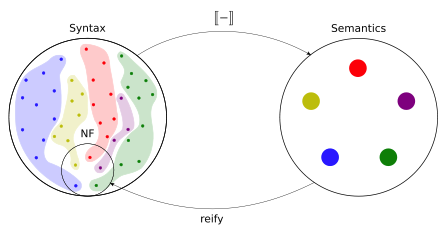
\includegraphics[width=0.6\textwidth]{./images/nbe_diagram}
    \caption{A visual overview of the NbE algorithm from \cite{slides}}
    \label{fig:nbeOverview}
\end{figure}

NbE proceeds in two steps. The first is to evaluate terms in the lambda calculus into a semantic set. In \ref{fig:nbeOverview} terms are represented by dots in the syntax set and the evaluation function is denoted by $\llbracket - \rrbracket$, which we refer to as \code{eval}. The second step is to \code{reify} the semantic value back into the normal form of the original term. Thus, the \code{normalise} function which maps terms to their normal forms is the composition of \code{eval} and \code{reify}

% property of eval
\ref{fig:nbeOverview} illustrates why NbE works. The key property of the \code{eval} function is that $\beta$-equal terms (represented by dots of the same colour in the syntax set) evaluate to the same semantic value. This ensures that $\beta$-equal terms normalise to the same normal form. The key property of the \code{reify} function is that the codomain of \code{reify} is the subset of normal forms, so \code{normalise} is guaranteed to return a normal form. 

The remainder of this chapter defines the data NbE operates on and functions to perform NbE in Haskell.

\section{Syntax}

\begin{lstlisting}
    type Name = String

    data Expr = ExpVar Name
              | ExpLam Name Expr
              | ExpApp Expr Expr
\end{lstlisting}

Inhabitants of the inductively-defined datatype \code{Expr} are well-formed terms of the untyped lambda calculus with strings as variables. The first argument of the lambda case introduces a new variable name bound in the function body defined by the second argument. For example, the identity function $\lambda x . x$ would be encoded as \code{ExpLam "x" (ExpVar "x")}.

\begin{lstlisting}
    data NormalForm = NfNeutralForm NeutralForm
                    | NfLam Name NormalForm

    data NeutralForm = NeVar Name
                     | NeApp NeutralForm NormalForm
\end{lstlisting}

We now define the target syntax of the \code{normalise} function, \code{NormalForm}. Note that \code{NormalForm} is inhabited by all the terms not containing $\beta$-redexes \cite{slides}, since the definition of \code{NeApp} only permits application on non-lambda terms, which are encoded as values of type \code{NeutralForm}.

\section{Semantics}

\begin{lstlisting}
    data V = Neutral NeutralV
           | Function (V -> V)

    data NeutralV = NeVVar Name
                  | NeVApp NeutralV V
\end{lstlisting}

% TODO: Mentional easy to define V -> V in Haskell, harder in other languages, motivating advantage of Haskell?

The semantic set \code{V} has a very similar structure to the set of normal forms, however lambda terms are replaced with Haskell functions of type \code{V} $\rightarrow$ \code{V}.
% TODO: Include following paragraph or not - not justified? 
The similarity simplifies \code{reify} as for some terms there are obvious translations from semantics to syntax. The replacement of lambda terms will be useful in evaluating $\beta$-redexes at the semantic level instead of the syntactic level. 

% TODO: Discuss using why don't use Neutral Form but establish our own datatype

\section{Evaluation}

Evaluation proceeds by pattern matching on the given term, and evaluating its constituent subterms. However, the semantic meaning of subterms can differ depending on which variables are bound by which lambda term. For example, in the terms $\lambda x . \lambda y . xy$ and $\lambda y . xy$, the semantic meaning of the $xy$ subterm is different. Thus, in addition to the term itself, \code{eval} needs information about the bound variables introduced by surrounding lambda terms. 

To keep track of which variables have been bound by surrounding lambda terms, we construct an environment datatype.

\begin{lstlisting}
    type Env = Map Name V
\end{lstlisting}

Each key of the map corresponds to a bound variable name, and its associated value is the semantic value representing the variable. The environment can be thought of as the scope each subterm is evaluated in. 
% TODO: Include or not - helpful or overly general waffle?
It expands as more variables are bound in deeper subterms.

\begin{lstlisting}
    eval :: Expr -> Env -> V
\end{lstlisting}

\code{eval} takes an expression and the environment to evaluate it in, pattern matches on the expression, and returns the interpretation of the term in the semantic set. We now discuss the implementation of each case of the pattern match.

\begin{lstlisting}
    eval (ExpVar x) env = case lookup x env of
        Just y -> y
        Nothing -> Neutral (NeVVar x)
\end{lstlisting}

In the variable case, we lookup the variable in the environment. If the variable was bound by a surrounding lambda term, the variable will be present in the environment, and we can return the semantic value associated with it. Otherwise, the variables is free, so we return a semantic variable with the same name.

\begin{lstlisting}
    eval (ExpLam var m) env = Function f where
        f v = eval m env' where
            env' = insert var v env
\end{lstlisting}

% TODO: Include or not, repeating code in words?
The semantic interpretation of a lambda expression is a Haskell function of type \code{V} $\rightarrow$ \code{V}. This function takes an element \code{v} of the semantic set \code{V}, and returns the body of the lambda evaluated in an extended environment \code{env'}. In this extended environment, we bind the named variable \code{var} to \code{v}.

From the variable case, we see that whenever the variable \code{ExpVar var} is evaluated in the function body it will be interpreted as \code{v}. We can think of \code{v} as a semantic placeholder for the value \code{f} is applied to (if any). The use of this approach is demonstrated in the application case.

\begin{lstlisting}
    eval (ExpApp m n) env = app (eval m env) (eval n env)

    app :: V -> V -> V
    app (Function f) v0 = f v0
    app (Neutral n)  v0 = Neutral (NeVApp n v0)
\end{lstlisting}

In the application case we evaluate the \code{m} and \code{n} terms in the same environment, before applying them to the \code{app} function, which handles the application of semantic values. 

In the case where the first value is a function \code{f}, we evaluate \code{f} at the second argument \code{v0}. From the lambda case we see that this subcase corresponds to evaluating a redex term. Instead of contracting the redex by substituting at the syntactic level, we evaluate it using function application at the semantic level. The application instantiates the placeholder \code{v} at the semantic value \code{v0} in the lambda body. 

% TODO: Explain more
In the case that the first value is a value \code{n} of type \code{NeutralV}, there is no redex to contract, so we return a placeholder Neutral application at the semantic level.

\section{Gensym Reification}

Reification proceeds by pattern matching on the semantic value. 

Since evaluating a lambda yields a function, reifying a function should yield a lambda to ensure that \code{normalise} preserves terms already in normal form. This introduces a question: what variable should the returned lambda term bind? The new bound variable should be different to all other bound variables in scope, otherwise \code{reify} could produce invalid terms. It should also be different to all other free variables in the original term, to prevent free variable capture. Since terms are considered equal up to bound variable renaming by $\alpha$-equivalence, we can choose any variable name that satisfies these requirements. 

\begin{lstlisting}
    type FreshName = State [Name]
\end{lstlisting}

\begin{lstlisting}
    reify :: V -> FreshName NormalForm
    reify (Neutral n)  = do 
        reifiedN <- reifyNeutral n
        return (NfNeutralForm reifiedN)
    reify (Function f) = do
        freshNames <- get
        -- Remove the first name from the freshNames stream
        let freshVar = head freshNames
        -- The first name is no longer fresh (we are abount to use it as a bound variable)
        -- Modify the state to remove the used variable name
        modify tail
        -- Reify the body of the semantic function when evaluated at the fresh bound variable
        normalForm <- reify (f (Neutral (NeVVar freshVar)))
        return (NfLam freshVar normalForm)

    reifyNeutral :: NeutralV -> FreshName NeutralForm
    reifyNeutral (NeVVar i)   = return (NeVar i)
    reifyNeutral (NeVApp n m) = do
        reifiedNeutral <- reifyNeutral n
        reifiedNormal  <- reify m
        return (NeApp reifiedNeutral reifiedNormal)
\end{lstlisting}


\begin{lstlisting}
    normalise :: Expr -> NormalForm
    normalise exp = evalState (reify (eval exp empty)) freshNames 
        where
            freshNames = (getFreshVariableStream . getFreeVariables) exp
\end{lstlisting}

\subsection{Fresh variables solution 1 - Gensym}
approach based on \cite{slides}

Implemented with State monad

Issue with solution 1: Have to add monad everywhere (inescapable) - all functions dependent on state

"Less functional" - carry around state (may as well use imperative)
\section{de Bruijn Reification}
\subsection{Fresh variables solution 2 - Locally nameless terms}
approach based on \cite{deBruijn}

Uses de Bruijn Indicies for syntax and deBruijn levels for semantics

index n references nth abstraction,
if m abstractions: if n < m bound variables, otherwise free variable

Shifting for abstractions
